\chapter{Introducción}
\label{cap:Introduccion}

El consumo de energía se ha convertido en una problemática cada vez más relevante en los últimos años. En primer lugar, los países en desarrollo dependen en gran medida de los combustibles fósiles, lo que puede generar tensiones geopolíticas por el acceso a estos recursos, además de causar inseguridad energética y volatilidad en los precios. En segundo lugar, la producción y el consumo de energía suelen ir acompañados de la emisión de contaminantes atmosféricos, como el dióxido de azufre y el dióxido de carbono, lo que deteriora la calidad del aire y afecta la salud, aumentando el riesgo de enfermedades respiratorias. Finalmente, el alto consumo de energía requiere la construcción de infraestructura adicional para satisfacer la demanda, provocando una pérdida grave de biodiversidad y efectos negativos en la flora y fauna.

Según \cite{electricidadEspana},  el precio medio del mega-vatio-hora (MWh) en España durante 2022 superó la barrera de los 200 euros. Estos resultados pueden observarse en la Figura~\ref{fig:precioMedioLuz}, los cuales arrojan una subida general en el coste de la electricidad en los últimos años. Es por ello que, en el contexto económico, el precio sea un factor cada vez más importante. Las razones de este incremento son varias, siendo actualmente la más destacable que la producción energética nacional no es capaz de satisfacer la demanda total, lo que obliga a importar energía procedente de otros países. También es destacable el coste relativo al mantenimiento y la actualización de la red eléctrica, repercutiendo en el precio final. En líneas generales: la energía es un recurso cada vez más crítico para el ser humano. 

\begin{figure}[H]
    \centering
    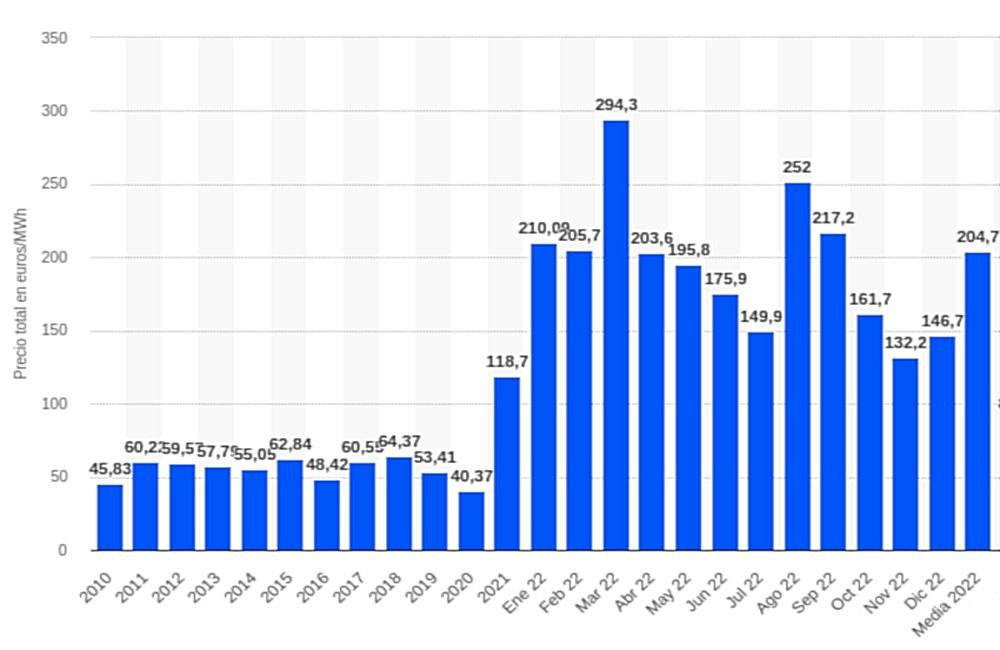
\includegraphics[width=0.85\linewidth, height=0.45\textwidth]{figs/electricidadStatista.jpg}
    \caption{Precios medios de electricidad en España entre 2010 y 2022~\cite{electricidadEspana}.}
    \label{fig:precioMedioLuz}
\end{figure}

En la actualidad, dentro del contexto de la informática, el consumo de energía también es una problemática tenida en cuenta, estando presente en todas las etapas de desarrollo, desde el diseño de arquitecturas, hasta la implementación a nivel físico. Este comportamiento se ha visto reforzado en los últimos años, debido a la creciente demanda de \ac{SoC}, un tipo de \textit{chip} que contiene toda o la mayor parte de los componentes requeridos por un dispositivo informático. Los \ac{SoC} están presentes en multitud de aparatos, como \textit{smartphones}, automóviles, o relojes inteligentes, entre otros. Estos dispositivos no están conectados a la red eléctrica de forma constante, sino que funcionan a base de baterías, siendo necesario minimizar el consumo para maximizar la vida útil de éstas. Esto ha desembocado en el desarrollo de \textit{hardware} y \textit{software} más eficientes a nivel energético. Según \cite{mercadoSoc}, la cuota de mercado mundial de sistemas en chip se estimó en 169,54 millones de dólares en el año 2023 y se prevé que crezca a una \ac{CAGR} del 8,5\% entre los años 2024 y 2030, mostrándose estos resultados en la figura \ref{previsionesSoc}. Un ejemplo real de dispositivo que integra un \ac{SoC}, en este caso, reloj inteligente, es el Xiaomi Watch 2, del año 2023, el cual puede verse en la figura \ref{xiaomiReloj}, con una batería de 495 mAh, que dura, según el fabricante, más de dos días y medio \cite{xiaomiWatch}.

\begin{figure}[H]
    \centering
    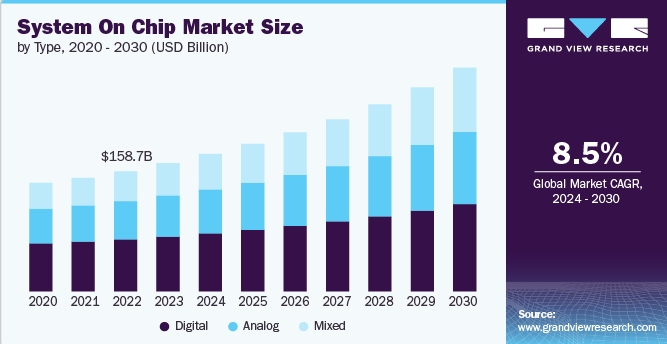
\includegraphics[width=0.95\linewidth, height=0.5\textwidth]{figs/graficaSoc.png}
    \caption{Previsiones cuota del mercado de SoC. Referencia: \cite{mercadoSoc}}
    \label{previsionesSoc}
\end{figure}

\begin{figure}[H]
    \centering
    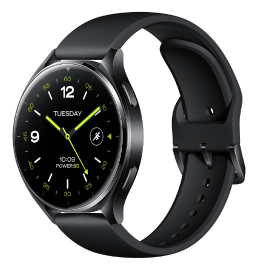
\includegraphics[width=0.3\linewidth, height=0.3\textwidth]{figs/relojinteligente.png}
    \caption{Xiaomi Watch 2. Referencia: \cite{xiaomiWatch}}
    \label{xiaomiReloj}
\end{figure}

En este contexto, para poder estimar el consumo global de la plataforma desarrollada es necesario realizar pruebas de todo tipo. Los fabricantes realizan estas comprobaciones de múltiples formas, como pruebas empíricas directamente sobre el \ac{IC}, o mediante simulaciones \textit{hardware} lo más parecidas posible a la plataforma física. Ambos procedimientos son capaces de generar un modelo de consumo de la plataforma fiable que permita estimar la energía empleada por la plataforma en cuestión, para poder validar el \textit{hardware} desarrollado. En el contexto de este \ac{TFM} se ha centrado el esfuerzo en el segunda opción, debido a la imposibilidad de realizar mediciones con precisión directamente sobre un \ac{IC}, si bien se han realizado pruebas con instrumental eléctrico sobre el cable de alimentación de la plataforma de cómputo.

Dentro del área del consumo de energía en sistemas informáticos, hay una serie de filosofías de diseño de arquitecturas \textit{hardware} enfocadas a este contexto, siendo \ac{RISC} la más destacable, y de sus muchos seguidores, a \ac{ARM}, la empresa dedicada a diseñar arquitecturas de bajo consumo líder a nivel mundial. En la acualidad, según \cite{mercadoArm}, esta empresa registró una participación de mercado superior al 90\% dentro del mercado de aplicaciones móviles, además de tener una participación del 65\% en el \ac{IoT}.

Este \ac{TFM} aborda la propuesta y validación de un modelo de consumo extensible a dispositivos con arquitecturas \textit{hardware} similares al Raspberry Pi 4 Model B, dispositivo \ac{SBC} basado en arquitectura \ac{ARM}, sobre el que se ejecutarán una serie de \textit{benchmarks} sintéticos, los cuales permitirán la obtención de resultados deterministas y detectar los componentes \textit{hardware} más relevantes dentro de la plataforma, para obtener una serie de métricas, con el objetivo de  que, siguiendo un marco de medición concreto, se pueda caracterizar el consumo energético del dispositivo en cuestión. Como resultado, este \ac{TFM} pretende ser la base para desarrollar una metodología en términos de consumo energético que permita definir una forma directa de determinar el consumo de ciertos componentes de una plataforma \textit{hardware} basándose en simulaciones de una pseudo-plataforma desarrollada con el programa Gem5, el cual se explicará en mayor detalle en los siguientes capítulos del trabajo. Fruto de este \ac{TFM}, se podría desarrollar, por ejemplo, un planificador de tareas para sistemas empotrados, enfocado en el ahorro energético gracias a las estimaciones de consumo por aplicación, permitiendo aumentar el tiempo de vida del sistema sin tener que realizar cambios. 

Para finalizar, se describe a continuación la estructura de este \ac{TFM}, que se divide en los siguientes capítulos:

\begin{enumerate}
    \item \textbf{Introducción}. Este capítulo es el actual, donde se ha tratado de dar una respuesta sobre la necesidad, desarrollo, y potenciales resultados del \ac{TFM} en cuestión.
    \item \textbf{Objetivos}, donde se plantearán el objetivo principal y los objetivos secundarios que han surgido conforme se ha desarrollado este \ac{TFM}. 
    \item \textbf{Estado del Arte}, capítulo en el cual se expondrá tanto el concepto como el estado actual de las tecnologías utilizadas, así como las herramientas necesarias en el trabajo.
    \item \textbf{Metodología}, donde se detallará la metodología seguida en el \ac{TFM}, así como los principales aspectos y etapas dentro de la misma.
    \item \textbf{Resultados}, capítulo que explicará en detalle, y siguiendo la metodología seleccionada previamente, el desarrollo del trabajo en cuestión, exponiéndose los resultados obtenidos en cada etapa. 
    \item \textbf{Conclusiones} donde se analizará si los resultados obtenidos satisfacen los objetivos principales y secundarios, planteados previamente. Asimismo, en este capítulo se propondrán propuestas para nuevos trabajos y se evaluarán las competencias adquiridas o reforzadas tras el desarollo de este trabajo.
    \item \textbf{Anexos (A,B,C)}, que contendrán las tablas y figuras que sean de menor relevancia, o que hayan sido imposible de colocar dentro del trabajo en cuestión, por cuestiones de límite de páginas para el desarollo del \ac{TFM}.
    
\end{enumerate}
